Next, we built the whole mixing console and tested it.
\phantom{ } We combined all the parts we had built in previous labs, in the order of signal sources, (one of which was a microphone and preamplifier,) summing amplifier, equalizer, and speaker. The whole circuit graph is shown in the figure[\ref{fig:fullcir}].\\
\begin{figure}[!htbp]
	\centering
	\begin{framed}
		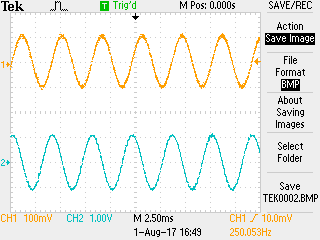
\includegraphics[width=\linewidth]{images/TEK0002.png}
		\caption{The waveform of the input and output signals}
		\label{fig:wave250}
	\end{framed}
\end{figure}

\begin{figure*}[!htbp]
	\centering
	\begin{framed}
		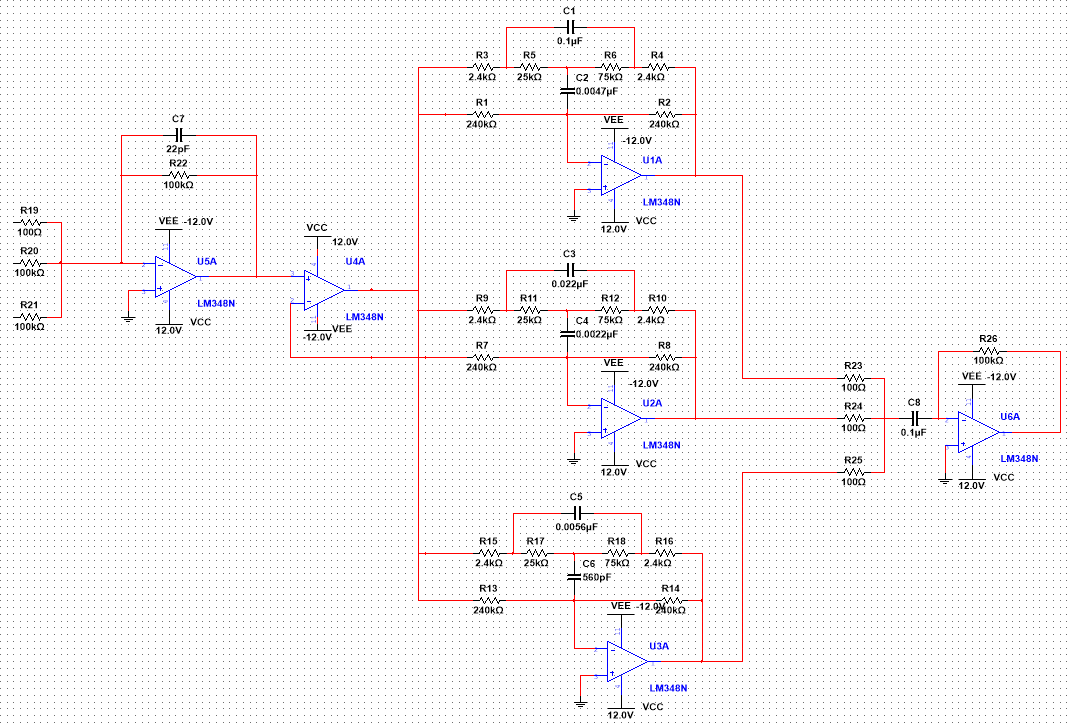
\includegraphics[width=\linewidth]{images/circ2.png}
		\caption{The audio mixer circuit}
		\label{fig:fullcir}
	\end{framed}
\end{figure*}
\phantom{ } Then we used a sine wave of 250Hz as an input to the system. The waveform of the input and output signals are shown in figure[\ref{fig:wave250}].\\
\hfill \newline
\textbf{Analysis\#3} \newline
\phantom{ } To determine which filter controls the amplitude of the output at 250Hz, we changed each of the potentiometers of the three filters. While two of them did not make any difference to the output wave form, when we adjusted $R_{23}$ in Fig[\ref{fig:fullcir}] to a lower resistance, the amplitude increased obviously. Since we only changed $R_{23}$, we can tell that the filter on the top controls the output at 250Hz, as expected. Since the 250Hz case overlaps with the requirement for a waveform above, more evidence is provided in the cases below.\\
\hfill \newline
\textbf{Analysis\#4} \newline
\phantom{ } Next, we used an input signal of 1kHz, and proved that the second filter controls the amplitude at this frequency. The three figures below show the change of output signal when the potentiometer was at 100\%, 50\% and 0\%, and we used Pk-Pk voltage to observe the amplitude changes. \\
\phantom{ } As the resistance of $R_{24}$ decreased, the amplitude of the output signal increased. Meanwhile, changing $R_{23}$ or $R_{25}$ did not make any difference to the waveform.\\
\newline
\phantom{ } The same was done with the 4kHz input. This time, we increased $R_{25}$ to see if everything changes in the same way. Figure[\ref{fig:wave4k}] displays the signals with the potentiometer at 0\%, 50\% and 100\%. We can see that the higher the resistance is, the lower the output amplitude goes. Still, the waveform did not change when we adjusted $R_{23}$ or $R_{24}$. Thus we proved that the filter on below, designed with a center frequency of 4kHz, controls the output amplitude here.

\begin{figure}[!htbp]
	\centering
	\begin{framed}
		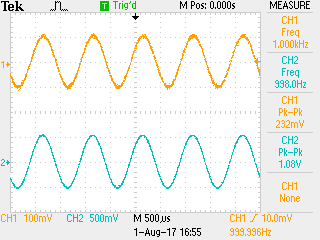
\includegraphics[width=\linewidth]{images/TEK0003.png}
		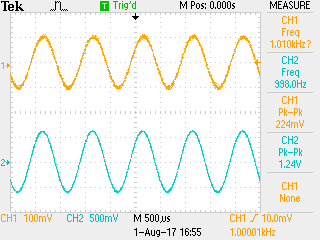
\includegraphics[width=\linewidth]{images/TEK0004.png}
		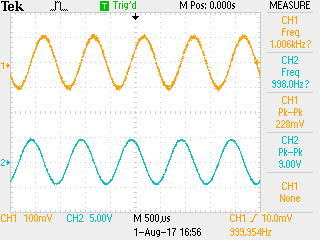
\includegraphics[width=\linewidth]{images/TEK0005.png}
		\caption{The changing of output signal at 1kHz}
		\label{fig:wave1k}
	\end{framed}
\end{figure}

\begin{figure}[!htbp]
	\centering
	\begin{framed}
		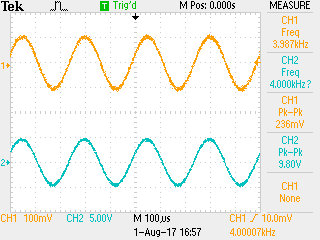
\includegraphics[width=\linewidth]{images/TEK0006.png}
		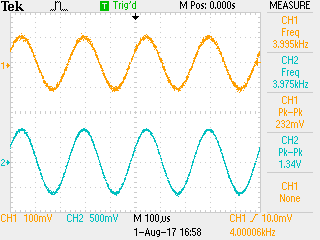
\includegraphics[width=\linewidth]{images/TEK0007.png}
		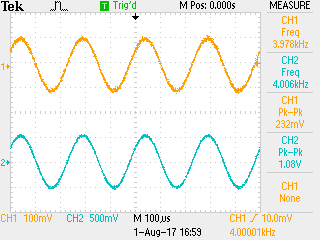
\includegraphics[width=\linewidth]{images/TEK0008.png}
		\caption{The changing of output signal at 4kHz}
		\label{fig:wave4k}
	\end{framed}
\end{figure}

\phantom{ } After we analyzed all three of the equalizer circuits, we then do tests using our audio mixer as a whole. We recorded the input and output amplitudes between 10Hz and 1MHz to plot the gain of the entire audio mixer. To avoid interference, we disconnected two other input channels. We also took down more data than required to find out how the curve goes above 4kHz. Our recorded data are shown in table[\ref{tab:datagain}], and are plotted in figure[\ref{fig:mixerg}].\\

\begin{table}[!htbp]
	\centering
	\caption{Measurements of the gain}
	\label{tab:datagain}
	\begin{tabular}{lccc}
		\toprule
		frequency($\si{\hertz}$) & $V_{in}$($\si{\milli\volt}$) & $V_{out}$($\si{\milli\volt}$) & gain($\si{\decibel}$) \\
		\midrule
		10	&224&	316&	2.98\\
		20	&220&	712&	10.2\\
		50	&220&	1680&	17.7\\
		100	&216&	2880&	22.5\\
		200	&220&	4000&	25.2\\
		500	&224&	4640&	26.3\\
		1000&	224&	4800&	26.6\\
		2000&	224&	4880&	26.8\\
		5000&	224&	4920&	26.8\\
		10000&	232&	4880&	26.5\\
		20000&	228&	4600&	26.1\\
		50000&	224&	3280&	23.3\\
		100000&	224&	1720&	17.7\\
		200000&	224&	608&	8.67\\
		500000&	224&	91.2&	-7.81\\
		1000000&	224&	24&	-19.4\\
		\bottomrule
	\end{tabular}
\end{table}

\begin{figure}[!htbp]
	\centering
	\begin{framed}
		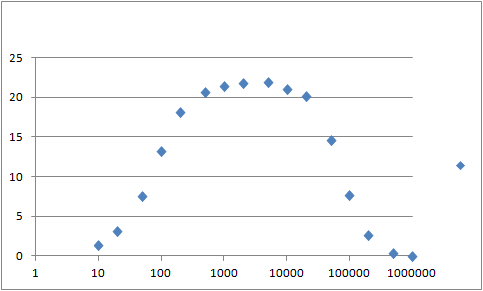
\includegraphics[width=\linewidth]{images/mixerg.png}
		\caption{The gain of the audio mixer}
		\label{fig:mixerg}
	\end{framed}
\end{figure}

\hfill \newline
\textbf{Analysis\#5} \newline